\chapter{软件透明的一致性协议及其证明}
\label{chap:protocol}

本章描述ThyNVM双模式检查点生成技术使用的基于状态机的数据一致性协议,以及协议的形式化证明。

\section{地址空间管理}

ThyNVM使用两个地址转换表,\emph{块转换表}(BTT)和\emph{页转换表}(PTT),来维护从物理地址空间到硬件地址空间的映射。

每个物理地址在NVM上有一个对应的固定的\emph{主硬件地址}。所以,确定一个物理地址的主硬件地址不需要经过BTT或PTT进行地址转换。不失一般性,我们假定主硬件地址和物理地址相等。与此同时,任何物理地址都可以通过BTT或PTT被\emph{动态地}映射到一个NVM上的不同的硬件地址,映射方式取决于ThyNVM检查点生成模式的规则。

为了方便内存管理,我们将硬件地址空间划分为六个有不同用途的区域。图~\ref{fig:addr-space-detail}描绘了ThyNVM地址空间的组织形式。下面我们描述每个区域的用途。

\begin{figure}[!h]
\centering
\includegraphics[width=0.7\linewidth]{addr-space-detail}
\caption{ThyNVM的物理和硬件地址空间。}
\label{fig:addr-space-detail}
\end{figure}


\textbf{家区域}:该区域位于NVM,包含所有主硬件地址。每个物理地址对应于一个本区域内的静态的主硬件地址。该区域的大小与物理地址空间的大小相同。

\textbf{块检查点区域}:该区域位于NVM,被BTT用来为检查点数据(\cl[block]或\cp[block])分配以缓存块大小为单位的存储空间。在块重映射模式中,一个块数据的工作副本(\wa[block])在其对应的BTT表项持久化后无需任何数据移动即可变为\cl[block]。所以,该区域同时保存着其BTT表项尚未持久化的\wa[block]数据。这样,一旦BTT完成持久化, 这些数据可以直接变成\cl[block]而不进行数据移动。

\textbf{页检查点区域}:该区域位于NVM,被PTT用来保存页粒度的检查点数据,即\cl[page]或\cp[page]。
家区域和页检查点区域交替保存\cl[page]和\cp[page]:如果\cp[page]保存在家区域中,那么\cl[page]则保存在本区域;反之亦然。

\textbf{页缓存区域}:该区域位于DRAM,是热点页工作副本(\wa[page])的缓存。在每个时间单元的检查点生成阶段,本区域中的脏页被回写到NVM作为\cl[page](位于上文描述的页检查点区域或家区域)。

\textbf{块缓存区域}:该区域位于DRAM,保存着一些块粒度的数据的临时副本。这些数据属于正在生成检查点的页。当程序执行和检查点生成过程重合时,对页缓存区域的写由块重映射模式处理,即被重映射到该区域做临时保存。

\textbf{BTT/PTT/CPU备份区域}:每个检查点生成阶段,BTT和PTT对应于{\cl}的版本都会保存在这个位于NVM中的区域。这样,当系统故障发生时,我们可以恢复出检查点数据所处的位置。检查点生成阶段开始时的CPU状态也保存在本区域,并与对应的BTT和PTT备份相关联。早于{\cp}版本的BTT/PTT/CPU备份可以被销毁。

这里的块检查点区域和页检查点区域共同对应于第\ref{subsec:thynvm-space}节描述的检查点区域A,而页缓存区域和块缓存区域则共同对应于工作数据区域。

\section{地址转换状态机}

我们使用一个状态机来决定一个内存写请求应当访问的位置,即将内存写请求的物理地址转换成一个合适的硬件地址。除了保存这个从物理地址到硬件地址的映射,每个BTT表项同时保存着7个状态之一,该状态驱动着块重映射模式的控制流。PTT重用与该状态机相同的逻辑,但只需要这些状态中的4个。下面我们聚焦于描述BTT的行为,而后讨论PTT如何适配到这个状态机的一个子集。图~\ref{fig-state-machine}描绘了状态机的全貌。为了清楚地展示,我们将状态分组而后逐组进行介绍。

\begin{figure}[!t]
\centering
\begin{tikzpicture}[->, >=stealth, node distance=0.37\tikzdistance, auto, thick,
font=\footnotesize, text centered]

\tikzstyle{every state}=[ellipse, inner sep=0pt]

\node[state] (h) [fill={rgb:black,1;white,4}] {\state{hidden}};
\node[state] (f) [right=of h, fill={rgb:black,1;white,4}] {\state{free}};
\node[state] (c) [above=of h, fill={rgb:black,1;white,4}] {\state{clean}};
\node[state] (t) [below left=of c] {\state{pre-hidden}};
\node[state] (d) [above=of f, fill={rgb:black,1;white,4}] {\state{dirty}};
\node[state] (s) [above right=of f] {\state{pre-dirty}};
\node[state] (l) [below right=of f] {\state{loan}};

\path (c.west)
  edge [bend right, anchor=south]
    node {\makecell[c]{write\\(ckpt.)\\\circled{$\mathnormal{6}$}}} (t);
\path (c)
  edge [anchor=east] node {\makecell[c]{write\\(exec.)\\\circled{$\mathnormal{3}$}}} (h)
  edge [anchor=west] node {\makecell[c]{revoke\\\circled{$\mathnormal{5}$}}} (f);
\path (h)
  edge [anchor=north] node {\makecell[c]{BTT flush\\\circled{$\mathnormal{4}$}}} (f)
  edge [loop, out=330, in=270, anchor=north, looseness=4]
    node [xshift=-0.05\tikzdistance] {write (exec.)} (h);
\path (t)
  edge [bend right, out=300, in=240, anchor=north]
    node [xshift=-0.1\tikzdistance] {\makecell[c]{write (exec.) $|$ clear\\\circled{$\mathnormal{7}$}}} (h)
  edge [loop, out=210, in=150, looseness=4, anchor=south]
    node [xshift=0.1\tikzdistance, yshift=0.15\tikzdistance]
      {\makecell[c]{write\\(ckpt.)}} (t);
\path (f)
  edge [anchor=west] node {\makecell[c]{write\\(exec.)\\\circled{$\mathnormal{1}$}}} (d)
  edge [bend right, anchor=base]
    node [xshift=0.12\tikzdistance, yshift=-0.05\tikzdistance] {\makecell[c]{\circled{$\mathnormal{8}$}\\write (ckpt.)}} (s)
  edge [bend right, anchor=base]
    node [xshift=-0.2\tikzdistance, yshift=-0.1\tikzdistance] {\makecell[c]{write\\to \region{Page Cache}\\(ckpt.)}} (l);
\path (s)
  edge [bend right, anchor=west]
    node [xshift=-0.15\tikzdistance, yshift=0.05\tikzdistance]
      {\makecell[c]{write (exec.) $|$ clear\\\circled{$\mathnormal{9}$}}} (d)
  edge [loop, out=330, in=30, anchor=north, looseness=4]
    node [xshift=-0.12\tikzdistance, yshift=-0.1\tikzdistance]
      {\makecell[c]{write\\(ckpt.)}} (s);
\path (d)
  edge node [anchor=south] {\makecell[c]{BTT flush\\\circled{$\mathnormal{2}$}}} (c)
  edge [loop, out=60, in=120, looseness=4, anchor=south]
    node {write (exec.)} (d);
\path (l)
  edge [bend right, anchor=west]
    node {\makecell[c]{write (exec.) $|$ clear\\\circled{$\mathnormal{10}$}}} (f)
  edge [loop, out=330, in=30, looseness=4, anchor=north]
    node [anchor=west] {\makecell[c]{write\\(ckpt.)}} (l);

\end{tikzpicture}


\caption{在块重映射模式下,一个BTT表项的状态。每个内存写(“write”)后注明“exec.”或“ckpt.”,分别意味着该内存写到来的时间在程序执行阶段(无检查点生成)或在检查点生成阶段;“write'”指原本应到页缓存的写。}
\label{fig-state-machine}
\end{figure}

\subsection{执行时的状态}

该组状态主要协调模式在程序执行(没有检查点生成)时的行为。为了决定内存写的正确地址,我们需要一个状态记录关于地址映射的两方面信息:(1)该物理地址在当前活跃时间单元内是否被写过。如果是的话,我们可以直接覆写对应的硬件地址,因为同一个时间单元内对相同物理地址的内存写可以合并。(2)硬件地址是一个主硬件地址还是位于检查点区域中。在某些情况下,如果我们需要避免覆写其中一个的话,我们将选择另外一个。据此,我们有四个状态来涵盖上述两个选择的所有组合。

\begin{itemize}
\item \textbf{\state{Free}态}:标志一个空的无有效映射的表项。同时我们将没有包含在BTT中的物理地址默认为\state{free}态。这意味着其物理地址在当前活跃时间单元内没有被更改过,且其检查点数据位于家区域中的主硬件地址。新来的对该物理地址的写请求必须在BTT中开辟一个新的表项将这个写重映射到块检查点区域。

\item \textbf{\state{Clean}态}:该状态表明其物理地址在当前活跃时间单元没有被更改过,且其检查点数据位于块检查点区域。新来的对该物理地址的写请求必须被BTT重映射到家区域的主硬件地址以保护检查点数据。

\item \textbf{\state{Dirty}态}:该状态表明其物理地址在当前活跃时间单元内被更改过,且对应的硬件地址在块检查点区域。该映射可以继续有效直到当前时间单元结束,用以合并到相同物理地址的内存写。在当前时间单元结束后,该硬件地址上的数据应当变为检查点数据,所以这个表项会被备份到NVM,将映射关系持久化,以备系统故障时定位检查点数据。

\item \textbf{\state{Hidden}态}:这个状态表明其物理地址在当前活跃时间单元内被更改过,且对应的硬件地址是位于家区域的主硬件地址。这里实际上并没有地址转换,因为主硬件地址和物理地址是相等的。然而,该表项会一直存在直到当前时间单元结束,目的是合并同时间单元内对该物理地址的其他写。在当前时间单元结束后,这个表项会被清除。


\vspace{\noindentsep}
\noindent \textbf{实例  }为了展示上述状态之间的动态转换,我们构造了图~\ref{fig-example}中的实例。我们首先忽略检查点生成期间的步骤(步骤A和B),并简单假设它们没有发生。在这个实例中,我们展示了三个连续的时间单元,记为时间单元0到2。从时间单元$k$收到的内存写会产生数据版本$v_k$,其中$k = 0, 1, 2$。

\begin{figure}[!ht]
\centering
\includegraphics[width=\linewidth]{figures/example.pdf}
\caption{连续时间单元中对物理地址P进行多次内存写的实例。}
\label{fig-example}
\end{figure}

\vspace{\noindentsep}
\noindent\ding{202} 初始状态,我们假设在物理地址P的数据位于其主硬件地址(家区域),所以在BTT中没有对应的表项,且不占用块检查点区域或块缓存区域的位置。P位置的数据可以认为是最近检查点的版本(标记为$v_{-1}$,即$v_0$之前的一个版本)。

\vspace{\noindentsep}
\noindent\ding{203} 在执行时间单元0的过程中,当一个对物理地址P的内存写到达时,我们不能覆写家区域中的检查点数据$v_{-1}$。所以,一个新的映射P-N被添加到BTT中,将数据$v_0$导向块检查点区域中的硬件地址N。我们将该表项标记为\state{dirty}态(图~\ref{fig-state-machine}中的状态转换\circled{$\mathnormal{1}$})以表明该物理地址在当前活跃时间单元内已经被更改过。这个时间单元内后续的任意对物理地址P的内存写都可以合并在硬件地址N。

\vspace{\noindentsep}
\noindent\ding{204} 在时间单元0之后,上述\state{dirty}表项被冲刷到BTT/PTT/CPU备份区域。该表项在BTT中的状态变为\state{clean}(状态转换\circled{$\mathnormal{2}$})以表明该映射已经持久化且在新的时间单元1中尚无对该物理地址的写。

\vspace{\noindentsep}
\noindent\ding{205} 时间单元0完成检查点生成之后,我们不再需要家区域中的数据$v_{-1}$。所以对物理地址P的内存写可以直接映射到主硬件地址。与此同时,相应的BTT表项状态变为\state{hidden}态(状态转换\circled{$\mathnormal{3}$})。该状态表明主硬件地址保存着数据$v_1$,而且这个时间单元内对P的后续写可以在这个位置上更新数据。如果这一步出现系统故障,ThyNVM则会回退到块重映射区域保存的数据$v_{0}$。

\vspace{\noindentsep}
\noindent\ding{206} 当时间单元2开始时,BTT冲刷操作已经将\state{hidden}状态清除,而这个表项被释放以表明家区域中的主硬件地址保存着物理地址P的数据的最近检查点版本$v_1$(状态转换\circled{$\mathnormal{4}$})。

我们可以看到,该BTT表项在连续多个时间单元收到内存写之后会变为\state{free}态。所以,多个时间单元之间的时间局部性可以减少使用中的表项,进而缓解对有限的BTT的存储空间的压力。在最坏状态下,如果BTT没有\state{free}状态的表项,我们必须撤销一个\state{hidden}态或者\state{clean}态的表项为新的内存写提供空间。\state{Hidden}态的表项无论如何都会在当前活跃时间单元结束时被撤销;
\state{Clean}态的表项可以被安全撤销(状态转换\circled{$\mathnormal{5}$})是因为他们不记录当前活跃时间单元内的新的更新。然而,被\state{clean}态表项引用的数据块(位于块检查点区域)需要和其主硬件地址上的数据互换。

\subsection{检查点生成时的状态}
\label{subsec:states-ckpt}

第二个状态组在检查点生成阶段发挥作用。该组包含两个状态,\state{pre-hidden}态和\state{pre-dirty}态,分别处理如下两种情况。

\begin{itemize}
\item
\textbf{\state{Pre-hidden}}态:该状态处理一个\state{clean}态的物理地址在检查点生成阶段收到内存写的情况。我们不能简单地像程序执行阶段一样执行状态转换\circled{$\mathnormal{3}$},因为家区域和块检查点区域的数据在检查点生成阶段都必须被保留。以图~\ref{fig-example}中的步骤A为例。因为我们当前处于时间单元1,块检查点区域的数据$v_0$是不可更改的,因为它是最近检查点 \cl 的一部分;同样地,家区域中的数据$v_{-1}$也不可更改,因为完整的一致的 \cl 尚未完成——如果此时系统故障终断了检查点生成进程,系统会回滚到$v_{-1}$(即 \cp)。因此,我们需要临时将工作数据(\wa)放入另外一个地方,块缓存区域,并相应地把这个特别的状态标记为\state{pre-hidden}(状态转换\circled{$\mathnormal{6}$})。\state{Pre-hidden}状态是\state{clean}状态和\state{hidden}状态之间的一个垫脚石。它只在当前活跃时间单元结束前存在。之后,如果该状态没有被一个内存写驱动转换到\state{hidden}(达到图~\ref{fig-example}中步骤4相同的结果),它会被显式地清理(状态转换\circled{$\mathnormal{7}$})。不论哪种情况,因为时间单元0的检查点(\cl)已经完成,版本$v_{-1}$(\cp)都会被工作数据 \wa 安全地覆写,并相应收回块缓存区域里 \wa 的位置。
\item
\textbf{\state{Pre-dirty}}态:该状态处理一个\state{free}态的物理地址在检查点生成阶段收到内存写的情况。与\state{pre-hidden}的处理逻辑类似,我们不能像程序执行阶段一样直接执行状态转换\circled{$\mathnormal{1}$}。以图~\ref{fig-example}中的步骤B为例。当时间单元1的检查点(\cl)正在生成的时候,我们不仅要保留$v_1$,还要保留$v_0$(\cp),因为 \cp 是我们仅有的完整一致的检查点。所以,我们把数据$v_2$放入块缓存区域,并向BTT添加一个\state{pre-dirty}态的表项来记录该映射(状态转换\circled{$\mathnormal{8}$})。\state{Pre-dirty}状态或者被下一个程序执行阶段的内存写命中转换到\state{dirty}态,或者在那个阶段结束时被清理转换到\state{dirty}态(状态转换\circled{$\mathnormal{9}$})。
\end{itemize}

因为\state{hidden}态和\state{dirty}态在每个检查点生成阶段刚刚开始时伴随BTT冲刷操作被清理,他们永远不会在检查点生成阶段与内存写相遇。所以,我们没有其他情况需要处理。

\subsection{用于双模式合作的状态}

最后我们有一个用于两个模式间合作的状态。当页回写模式生成脏页的检查点时,对这些页的各个内存写暂由块重映射模式重定向到块缓存区域(与第\ref{subsec:states-ckpt}节介绍的操作类似)。我们不把这些BTT表项混入上文的那些状态和转换,所以这些表项被标记为\state{loan}。当检查点生成结束这些页面重新可以被直接修改的时候,\state{Loan}态的表项最终将数据移回原页中(状态转换\circled{$\mathnormal{10}$})。

\section{问题定义}

本节给出协议证明的问题定义。我们这里聚焦于ThyNVM检查点生成模式的故障时一致性,亦即可恢复性——任何时候系统发生故障,ThyNVM可以恢复最近的一致的检查点。特别地,假设$t_k$为时间单元$k$结束执行的时刻,那么在$t_{k-1}$和$t_k$之间,ThyNVM顺次经历两个时间阶段,即一个检查点生成阶段(与时间单元$k+1$的程序执行阶段重合)和一个程序执行阶段(指没有与检查点生成重合的部分);$t_k$时刻的数据快照记为版本$v_k$,亦即时间单元$k$的检查点版本。我们将证明如下两个不变式,在状态机的转换中一直保持成立。

\textbf{不变式1}:在时刻$t_{k-1}$与$t_k$之间的检查点生成阶段,数据版本$v_{k-1}$和$v_{k-2}$及其在地址转换表中的映射都被保留。

Invariant 2: 在时刻$t_{k-1}$与$t_k$之间的程序执行阶段,数据版本$v_{k-1}$及其在地址转换表中的映射都被保留。

显然,如果上述两个不变式成立,那么系统在检查点生成阶段或程序执行阶段发生故障时,可以分别恢复到{\cp}或{\cl}。

\section{系统抽象}

\subsection{数据结构的抽象}

\subsection{程序行为的抽象}

\section{证明步骤}

\end{itemize}

